% \setchapterpreamble[u]{\margintoc}
\chapter{Introduction et résumé en français}
\labch{french}

\warn{
  This chapter is the French translation of \nrefch{intro}.
  You can also skip to the \hyperlink{toc}{table of contents}.
}

\selectlanguage{french}

La théorie des types se trouve à l'interface entre programmation et logique
formelle, les deux mondes se nourissant l'un l'autre. Des assistants de preuve
peuvent être basés dessus, ce qui en fait également des langages de
programmation à part entière, avec l'avantage supplémentaire de produire des
programmes certifiés.

Mon intérêt principal réside dans l'étude de la théorie des types tout en s'appuyant sur les outils qu'elle fournit :

My main interest lies in the study of type theory while relying on the tools it
provides: j'étudie la théorie des types \emph{au sein même} de la théorie des
types.
Ainsi, je me suis concentré sur la formalisation de la théorie des types dans
l'assistant de preuve \Coq~\sidecite[-0.7cm]{coq} et particuliètement sur
deux points:
\marginnote[0.7cm]{
  La \emph{reflection} et la notion d'égalité faible sont définies en
  \arefsubsecfr{ett-def} et \arefsubsecfr{wtt} respectivement, les deux dans
  le \refch{flavours}.
}
\begin{itemize}
  \item Comment peut-on transformer efficacement une preuve utilisant une notion
  très forte d'égalité appelée \emph{reflection}, en une preuve s'appuyant sur
  une notion très faible d'égalité ?
  \item Comment peut-on accroître la confiance dans notre système, dans mon
  cas \Coq, en utilisant ce système lui-même comme cadre pour l'étudier ?
\end{itemize}

\paradot{Contributions}
Mes contributions se trouvent principalement dans \avrefpart{elim-reflection}
et \avrefpart{coq-in-coq}, correspondant aux publications
suivantes~\sidecite{winterhalter:hal-01849166,sozeau2019coq,sozeau:hal-02167423}.
Bien que les chapitres précédant ces deux parties soient principalement
introductifs et correspondent à un état de l'art approximatif, ils contiennent
en réalité d'autres contributions, à savoir le travail que j'ai fait avec Andrej
Bauer sur le modèle cardinal dans \nrefch{models} actuellement non publié, et le travail avec Andrej Bauer et Philipp Haselwarter sur la formalisation de la
théorie des types appelée \ftt~\sidecite[-0.1cm]{formaltypetheory} et que je
présente brièvement dans \nrefch{formalisation}.

\marginnote[1.6cm]{
  On dit souvent ``assistant de preuve'', et je vais également le faire, mais il
  semblerait que la formulation ``assistant à la preuve'' soit plus correcte.
}%
\section{Assistans à la preuve}

L'un de mes objectifs est d'améliorer et de mieux comprendre les assistants de
preuve, mais qu'est-ce qu'un assistant de preuve?
Je pense que nous pouvons les voir comme des chatbots --- c'est-à-dire des
programmes avec lesquels vous pouvez converser --- qui sont là pour vous aider à
énoncer et à prouver des théorèmes.
Ils ne sont pas particulièrement intelligents et ne feront pas le travail pour
vous, mais ils sont très ennuyeux car ils ne comprennent pas toujours ce que
vous dites et vous devez être très précis ou ils vous feront remarquer vos
erreurs.

\marginnote[1.2cm]{
  L'utilisateur aura des bulles bleues, légèrement à gauche, tandis que
  l'assistant de preuve répondra en vert (réponse positive) ou en rouge
  (réponse négative) sur le côté droit.
}%
\begin{center}
  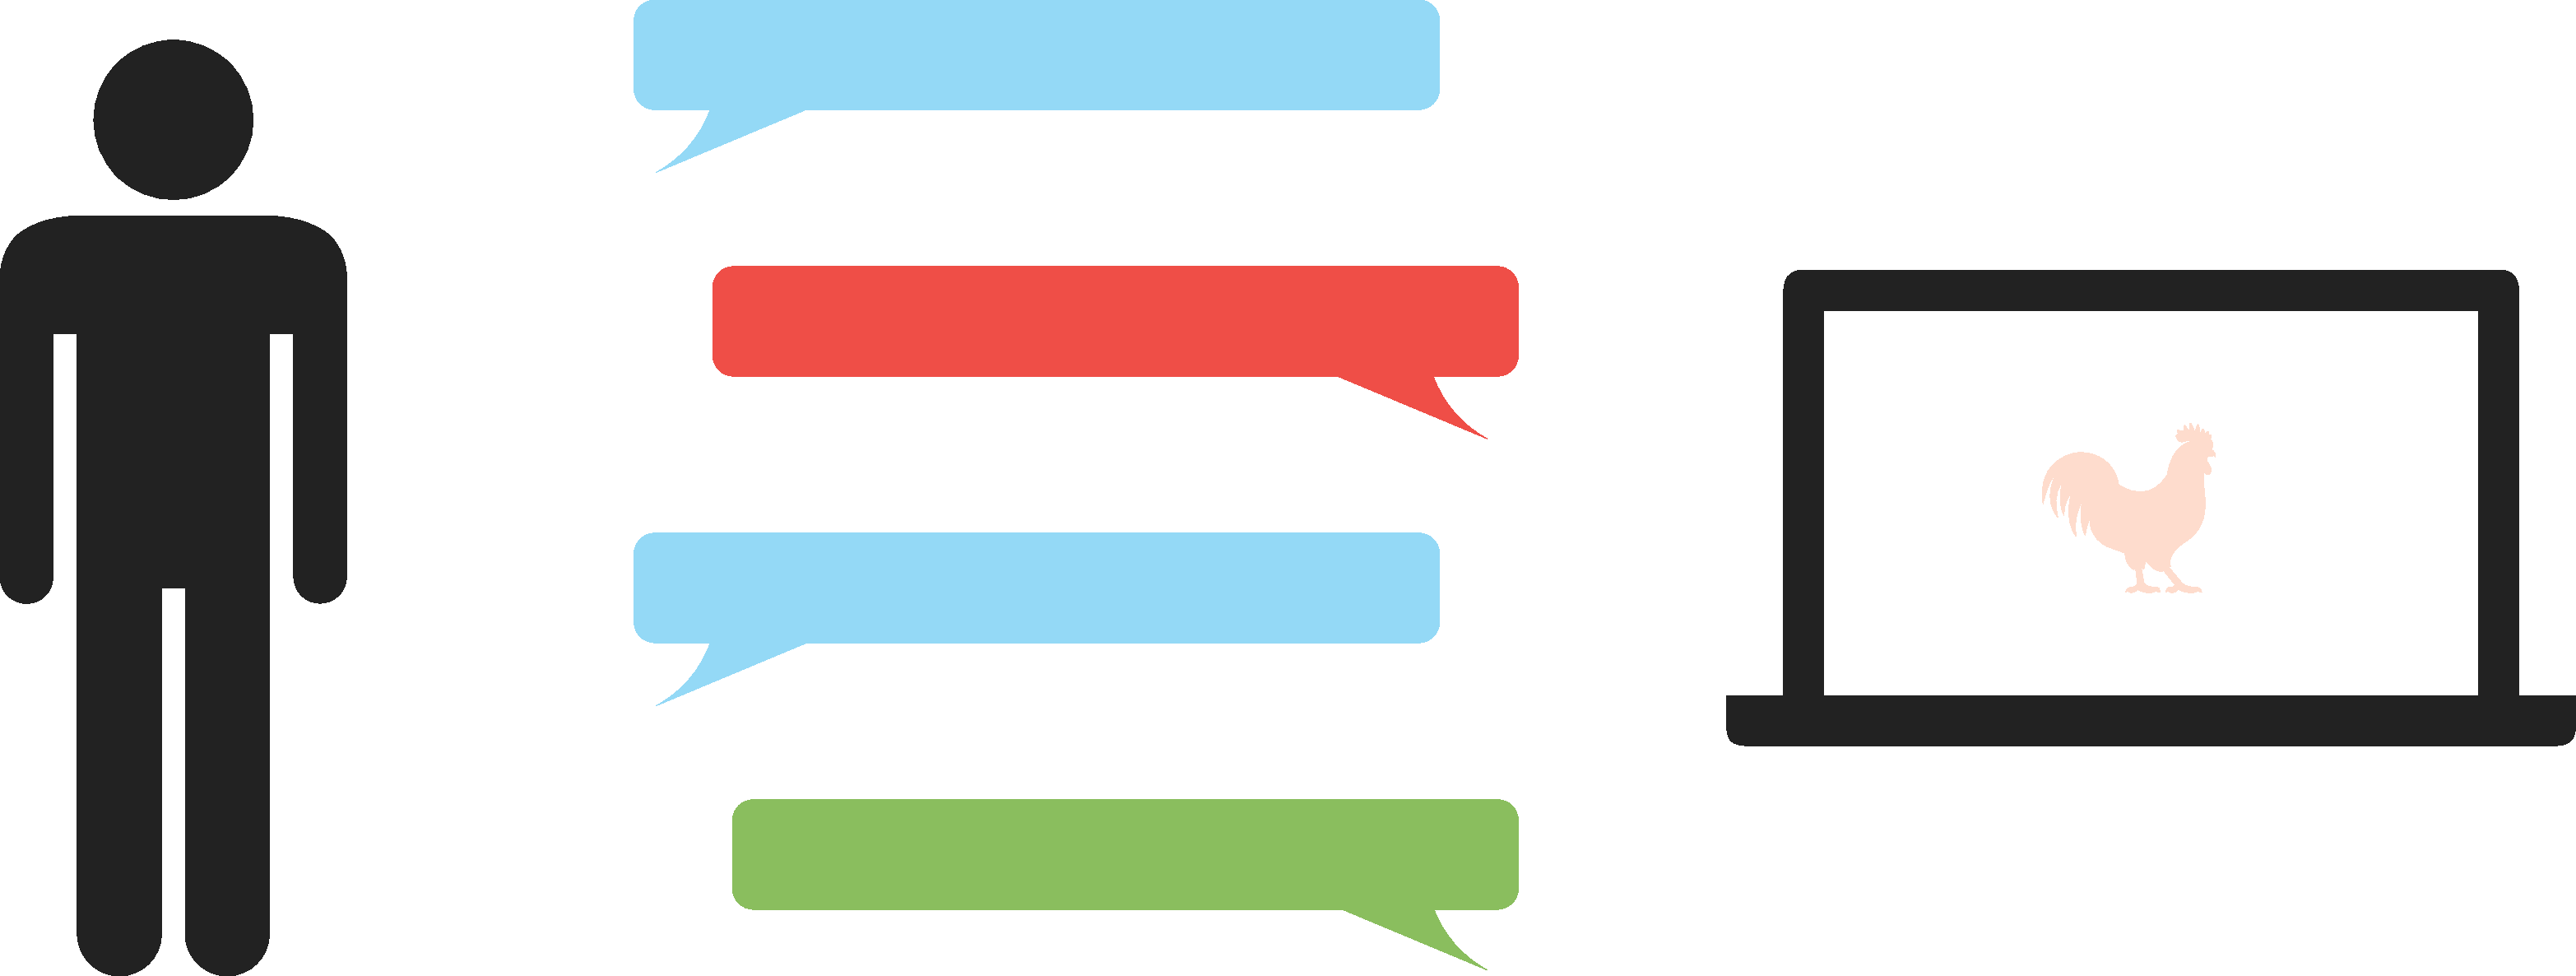
\includegraphics[width=0.6\textwidth]{coq-chatbot.pdf}
\end{center}

Ici, je représente l'utilisateur à gauche, en conversation avec l'assistant
de preuve, à droite, que j'imagine comme un ordinateur portable avec un coq à
l'intérieur.

Voyons maintenant en détail comment une telle conversation peut se dérouler.

\begin{center}
  
\includegraphics[width=0.8\textwidth]{modern-art.pdf}
\end{center}

\marginnote[0.1cm]{
  Quand je dis qu'ils sont d'accord, je veux dire que, en particulier,
  l'assistant de preuve a des connaissances de base sur les chats et les boîtes,
  par exemple, vous n'avez pas besoin de montrer qu'un chat est un félin.
  Il sait également ce que contient chaque boîte, par exemple que la quatrième
  boîte contient un chat rouge.
}
Cette œuvre d'art moderne sera le cadre de l'échange entre l'utilisateur et
l'assistant de preuve, et nous supposerons qu'ils sont tous les deux d'accord
sur ce cadre.
Nous avons des chats dans des boîtes (bien que l'un des chats soit plutôt un
lion), de différentes couleurs et soumis à différentes forces de gravitation.

Au début, l'utilisateur fait connaître son but à l'assistant de preuve, en
disant pour quel théorème il a besoin de son aide.

\begin{center}
  
\includegraphics[width=0.8\textwidth]{iwanterror-fr.pdf}
\end{center}

La phrase ci-dessus ne ressemble pas à un énoncé que nous pouvons prouver, et
l'assistant de preuve se plaindra à juste titre.

\begin{center}
  
\includegraphics[width=0.8\textwidth]{error-incomplete-fr.pdf}
\end{center}

En effet, nous sommes allé trop vite et avons oublié la moitié de ce que nous voulions dire. Cette fois, on lui donne une phrase complète.

\begin{center}
  
\includegraphics[width=0.8\textwidth]{iwant-is-fr.pdf}
\end{center}

Maintenant, l'énoncé est légèrement incorrect, ou pas assez précis pour notre
gentil assistant.

\begin{center}
  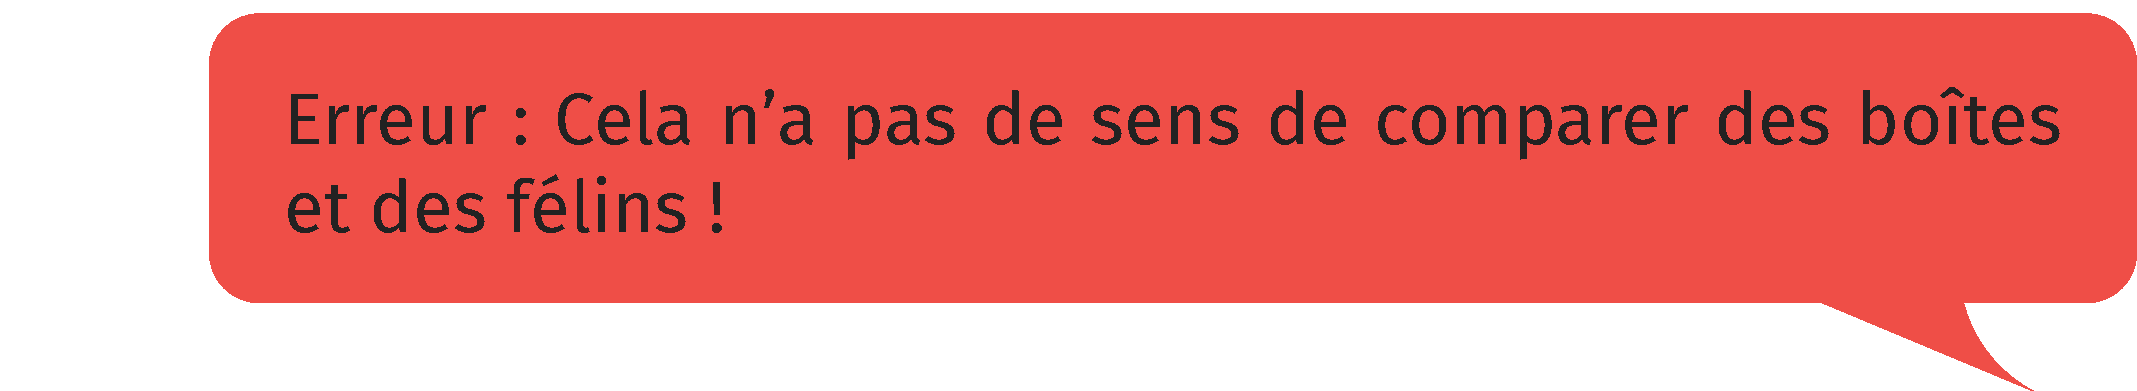
\includegraphics[width=0.8\textwidth]{error-box-feline-fr.pdf}
\end{center}

Nous devons réviser le théorème voulu et réaliser que nous ne voulons pas
prouver que toutes les boîtes sont des félins, bien qu'un humain puisse
comprendre ce que nous entendons par là, mais que toutes les boîtes
contiennent, chacune, un félin.

\begin{center}
  
\includegraphics[width=0.8\textwidth]{box-contains-feline-fr.pdf}
  
\includegraphics[width=0.8\textwidth]{how-to-prove-fr.pdf}
\end{center}

L'assistant de preuve a maintenant compris ce que nous voulions dire. La partie
interactive de la preuve commence maintenant. Nous voulons prouver une propriété
sur les boîtes, comme il y en a quatre à considérer, nous pouvons dire à
l'assistant de preuve que nous avons l'intention d'examiner chaque cas, un par
un.

\begin{center}
  
\includegraphics[width=0.8\textwidth]{convo7-fr.pdf}
  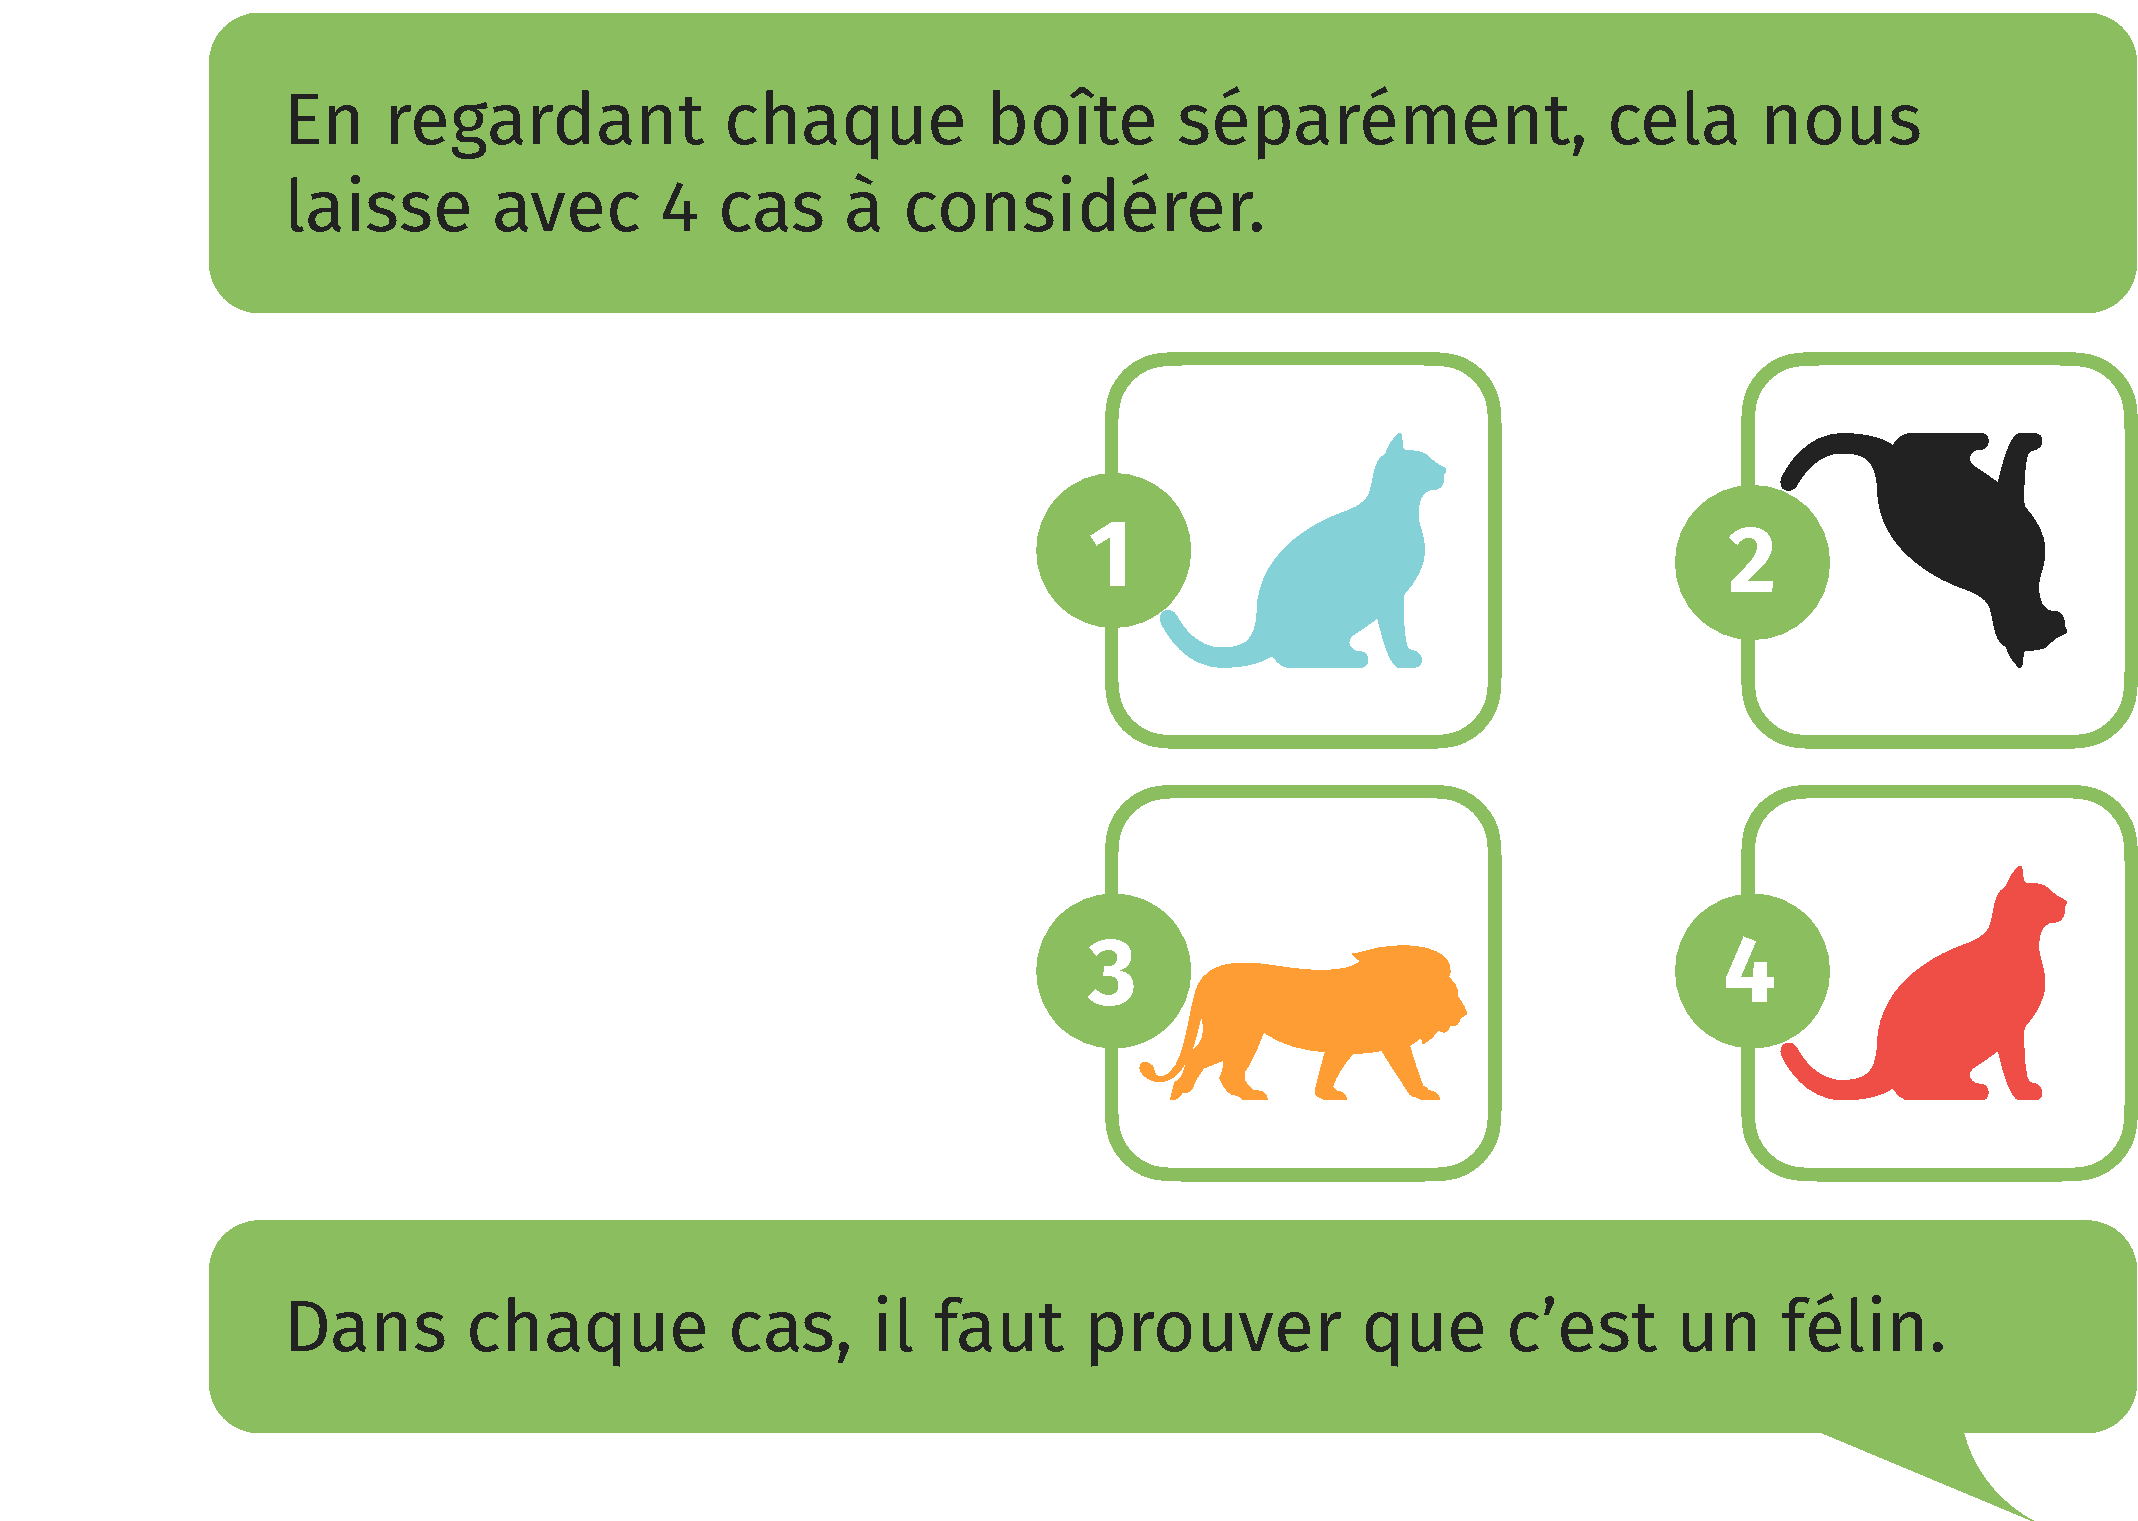
\includegraphics[width=0.8\textwidth]{convo8-fr.pdf}
\end{center}

On nous présente quatre cas, et autant d'énoncés à prouver.
Dans ce cas, nous sommes plutôt paresseux, d'autant plus que les quatre cas
seront similaires. Heureusement pour nous, l'assistant de preuve est capable de
comprendre que nous voulons traiter plusieurs cas de manière similaire,
\emph{et} est également capable de faire des preuves très basiques sans
l'intervention de l'utilisateur.

\begin{center}
  
\includegraphics[width=0.8\textwidth]{convo9-fr.pdf}
  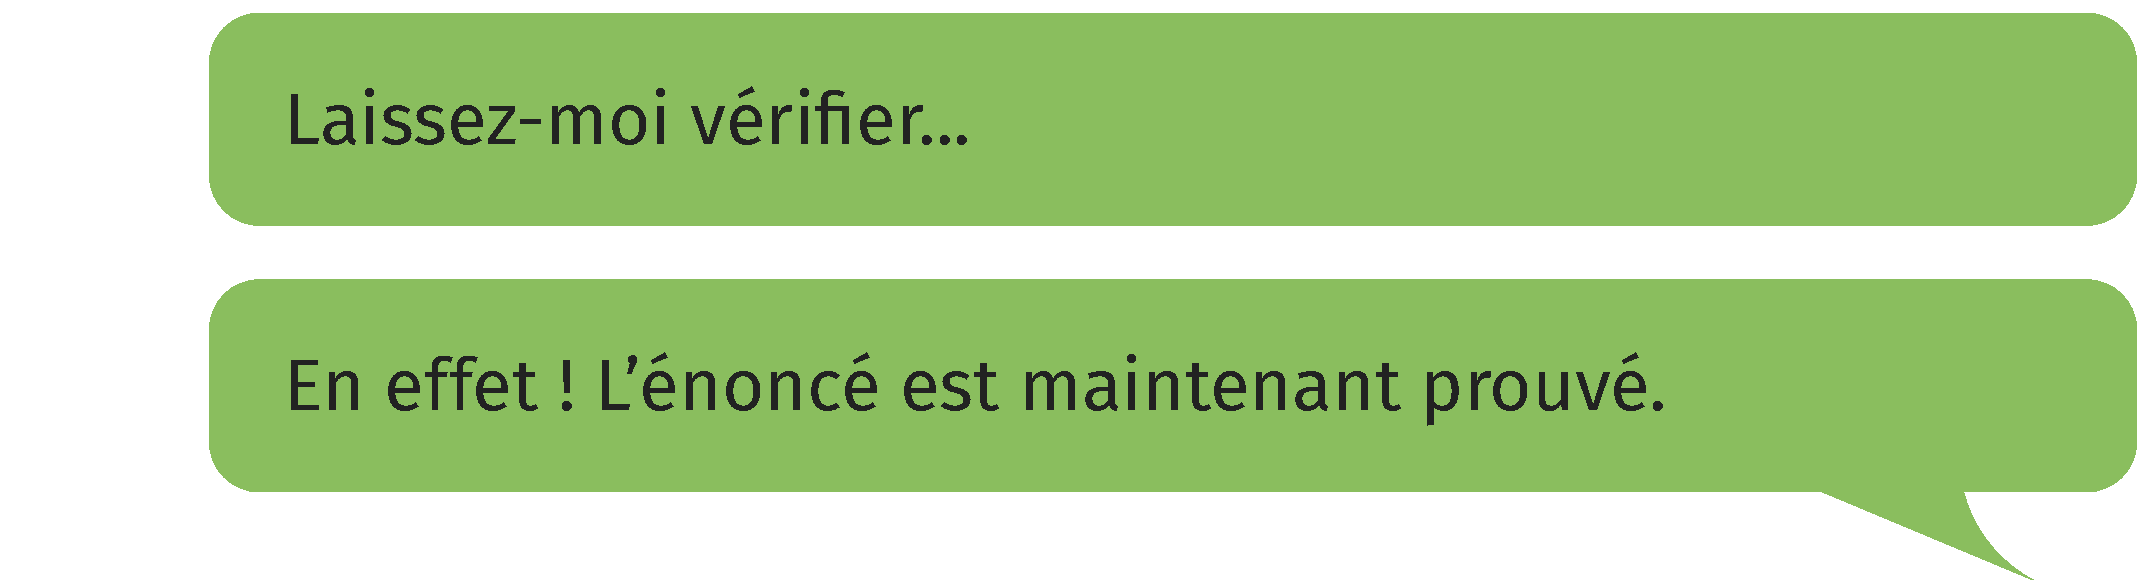
\includegraphics[width=0.8\textwidth]{convo10-fr.pdf}
\end{center}

Une fois la preuve terminée, l'assistant de preuve vous le dit et vous pouvez
passer à d'autres théorèmes pour le prouver. J'ai déjà montré que vous devez
être explicite et non ambigu lorsque vous parlez à l'assistant de preuve. Vous
devez également être correct.
L'assistant de preuve ne se fiera pas aveuglément à ce que vous dites.
%
Considérons maintenant un théorème qui n'est pas prouvable.

\begin{center}
  
\includegraphics[width=0.8\textwidth]{convo11-fr.pdf}
  
\includegraphics[width=0.8\textwidth]{how-to-prove-fr.pdf}
  
\includegraphics[width=0.8\textwidth]{convo7-fr.pdf}
  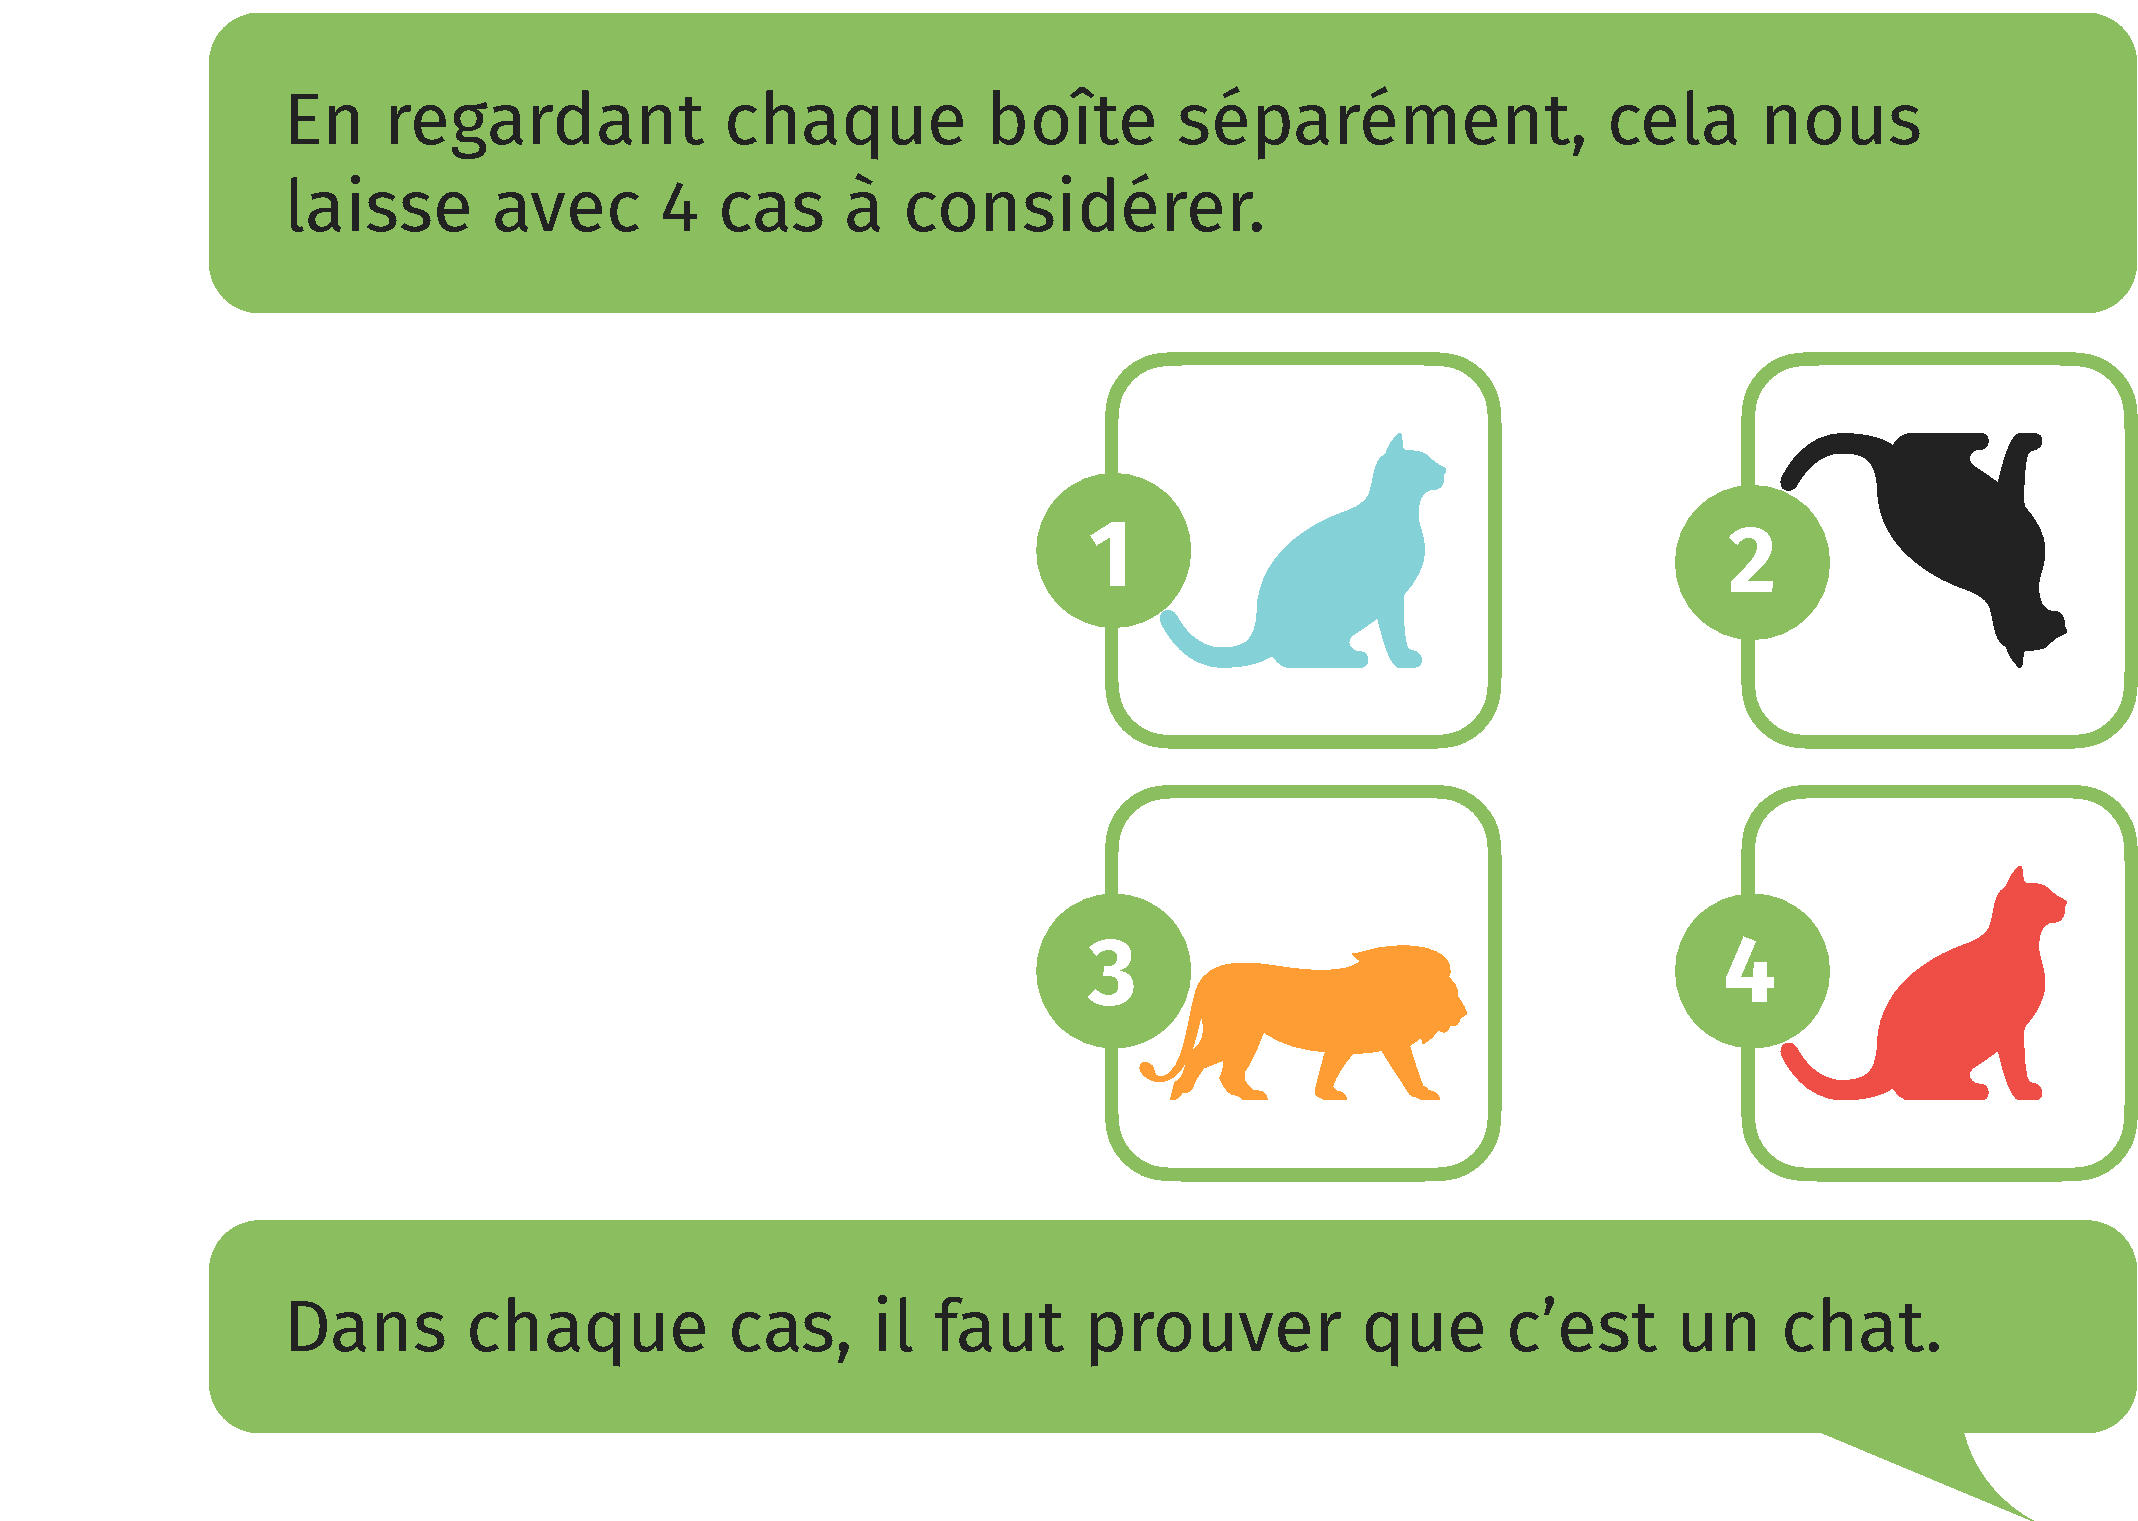
\includegraphics[width=0.8\textwidth]{convo12-fr.pdf}
  
\includegraphics[width=0.8\textwidth]{convo9-fr.pdf}
  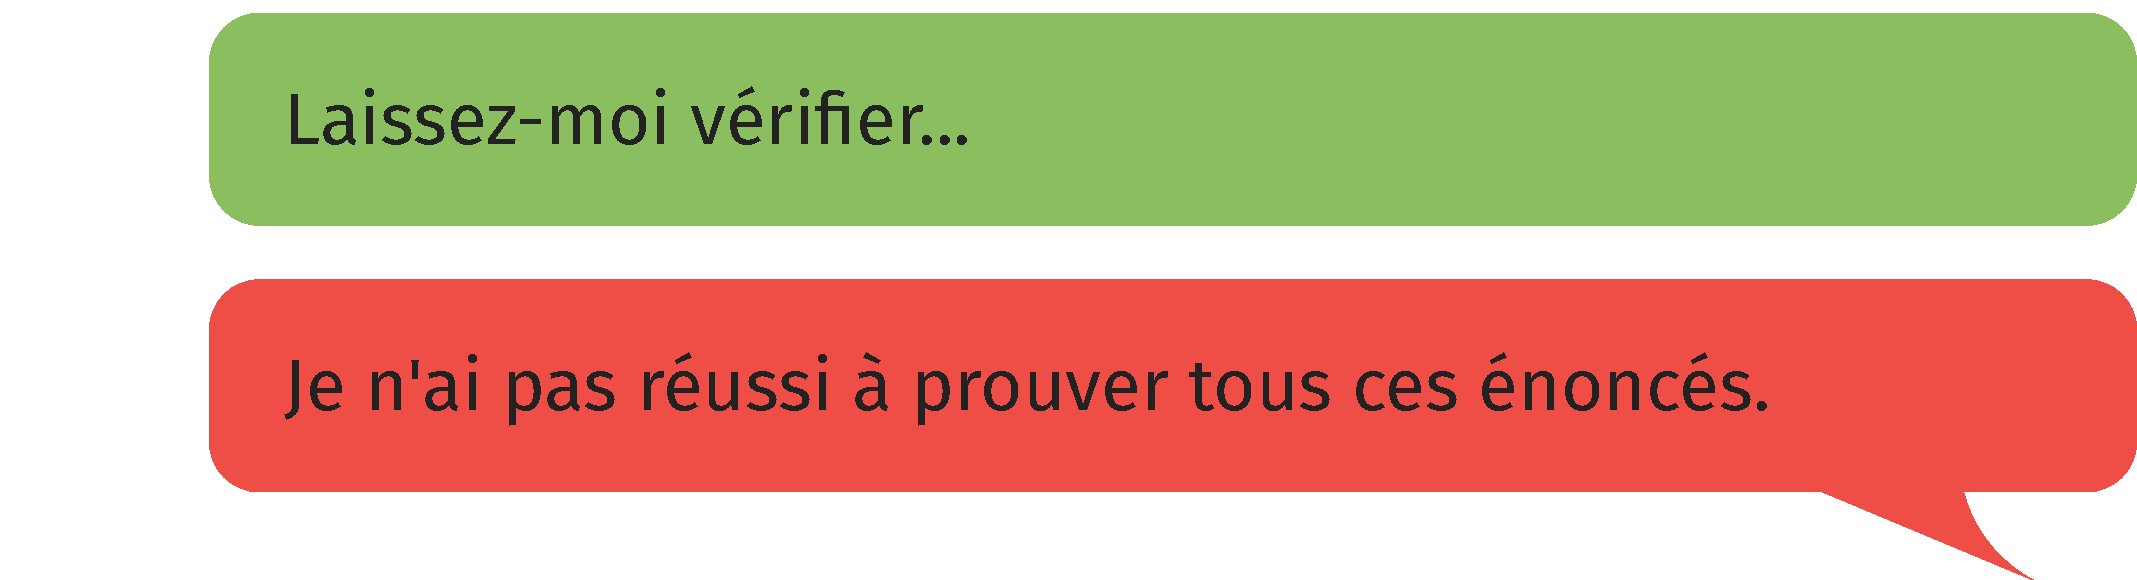
\includegraphics[width=0.8\textwidth]{convo13-fr.pdf}
\end{center}

Ici, l'assistant de preuve nous dit que tous les cas ne sont pas triviaux, nous
décidons donc de les examiner un par un pour comprendre ce qui ne va pas.

\begin{center}
  
\includegraphics[width=0.8\textwidth]{convo-focus-fr.pdf}
  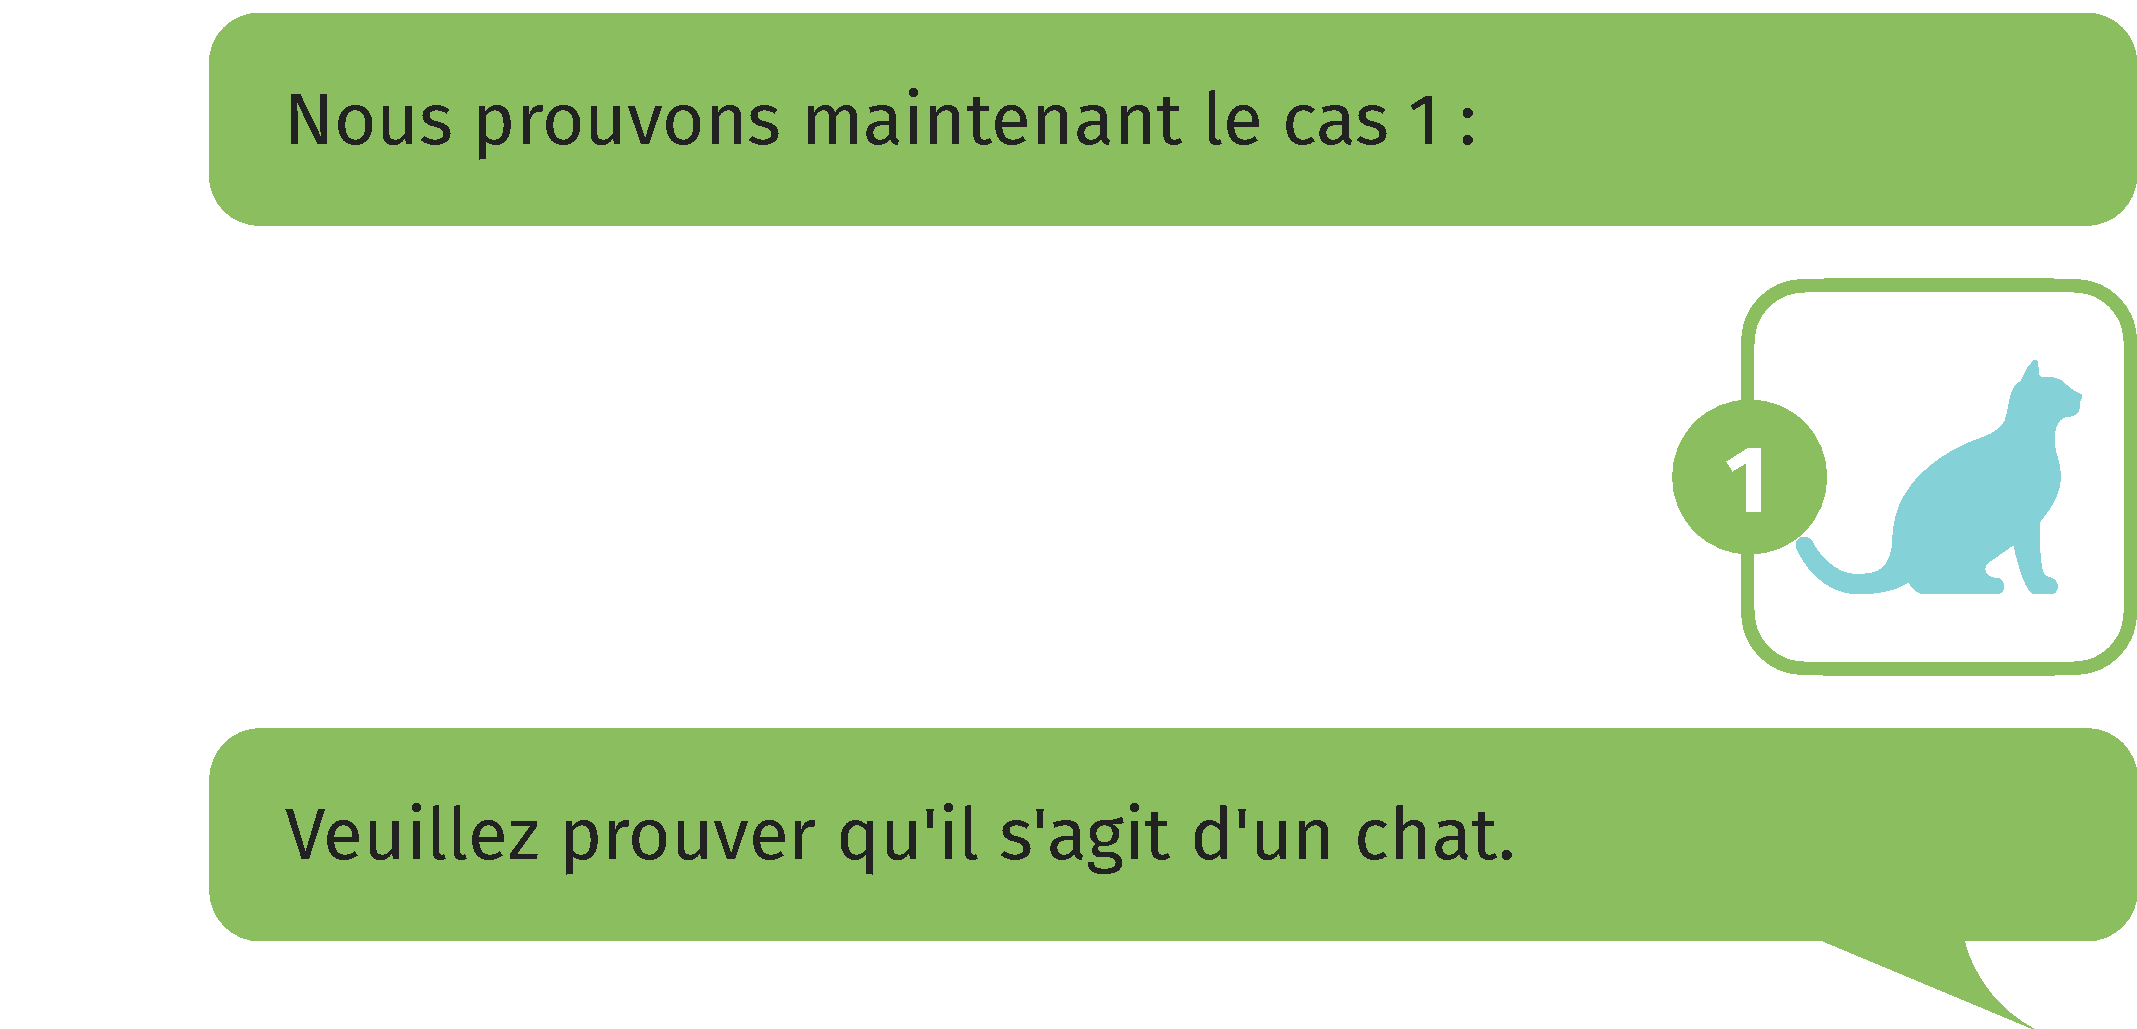
\includegraphics[width=0.8\textwidth]{convo-case1-fr.pdf}
\end{center}

Lorsque nous nous concentrons sur un cas, l'assistant de preuve nous rappelle ce
que nous devons prouver spécifiquement. Ici, nous revenons à l'utilisation de
notre stratégie antérieure et disons simplement que c'est évident.

\begin{center}
  
\includegraphics[width=0.8\textwidth]{convo-trivial-fr.pdf}
  
\includegraphics[width=0.8\textwidth]{convo-indeed-fr.pdf}
  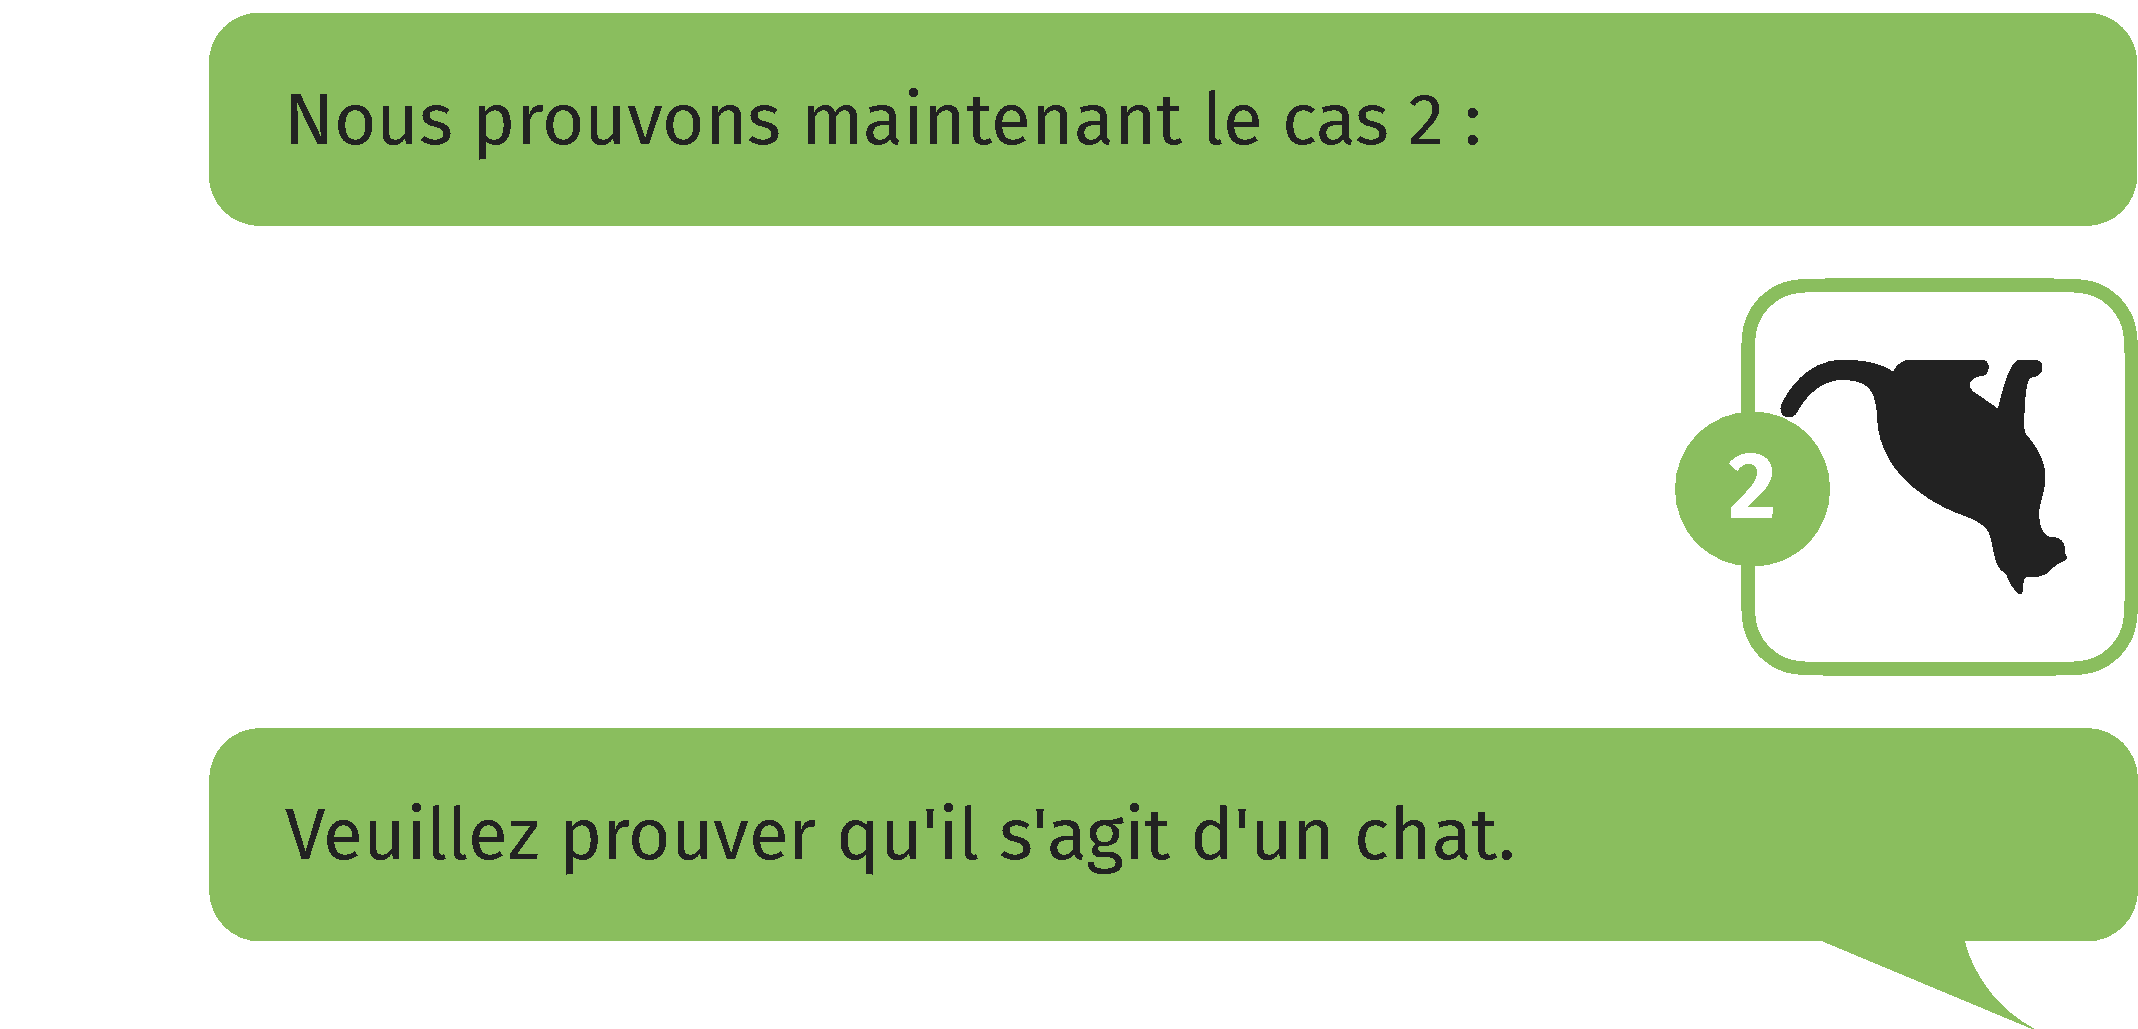
\includegraphics[width=0.8\textwidth]{convo-case2-fr.pdf}
  
\includegraphics[width=0.8\textwidth]{convo-trivial-fr.pdf}
  
\includegraphics[width=0.8\textwidth]{convo-indeed-fr.pdf}
  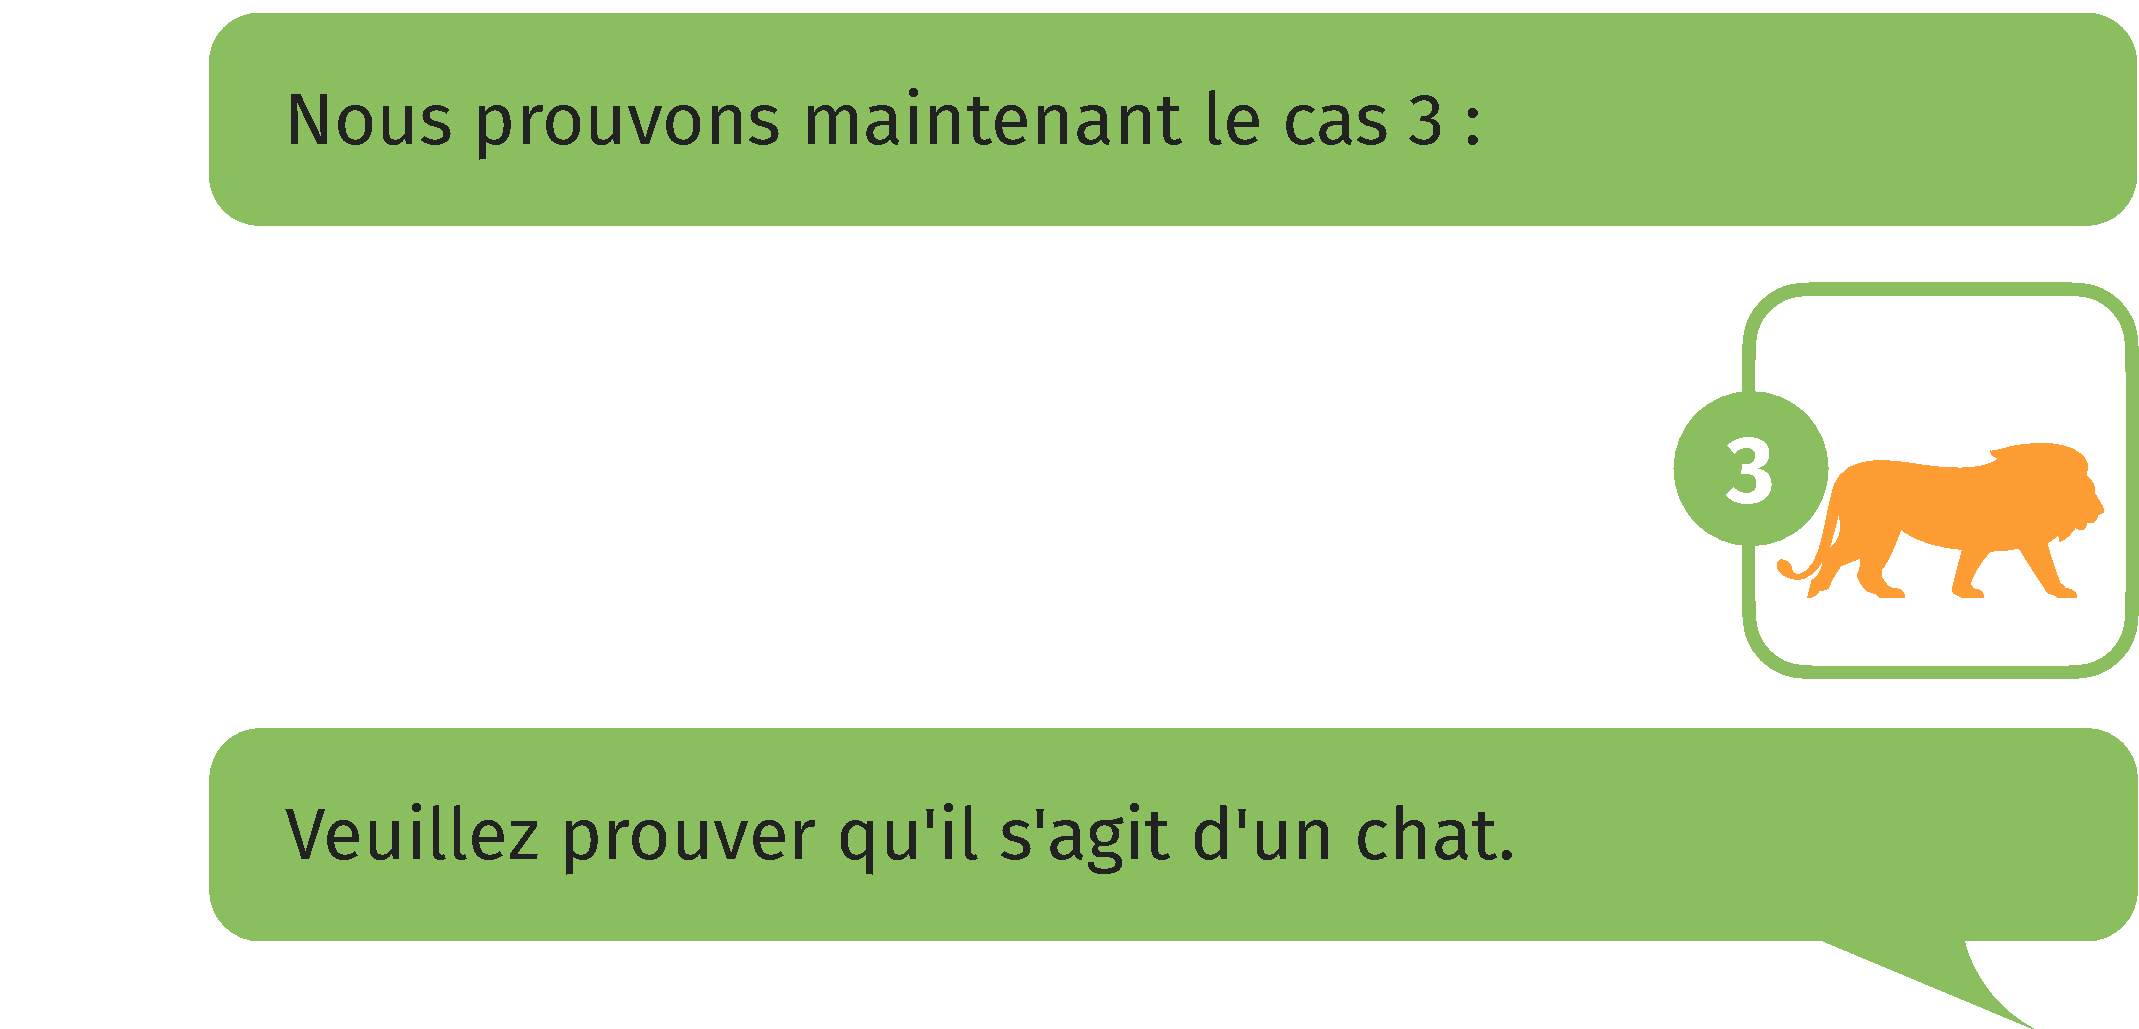
\includegraphics[width=0.8\textwidth]{convo-case3-fr.pdf}
  
\includegraphics[width=0.8\textwidth]{convo-abort-fr.pdf}
\end{center}

Cette fois, nous voyons que nous n'avons pas de chat donc nous n'essayons même
pas de le prouver.
Nous abandonnons la preuve, c'est-à-dire que nous renonçons à prouver un
énoncé que nous savons maintenant faux.
Une chose importante à noter ici est que l'assistant de preuve ne sait toujours
pas que l'énoncé est incorrect, mais seulement que la tentative de preuve était elle-même invalide.
Nous pouvons montrer que l'énoncé est faux en prouvant l'inverse :

\begin{center}
  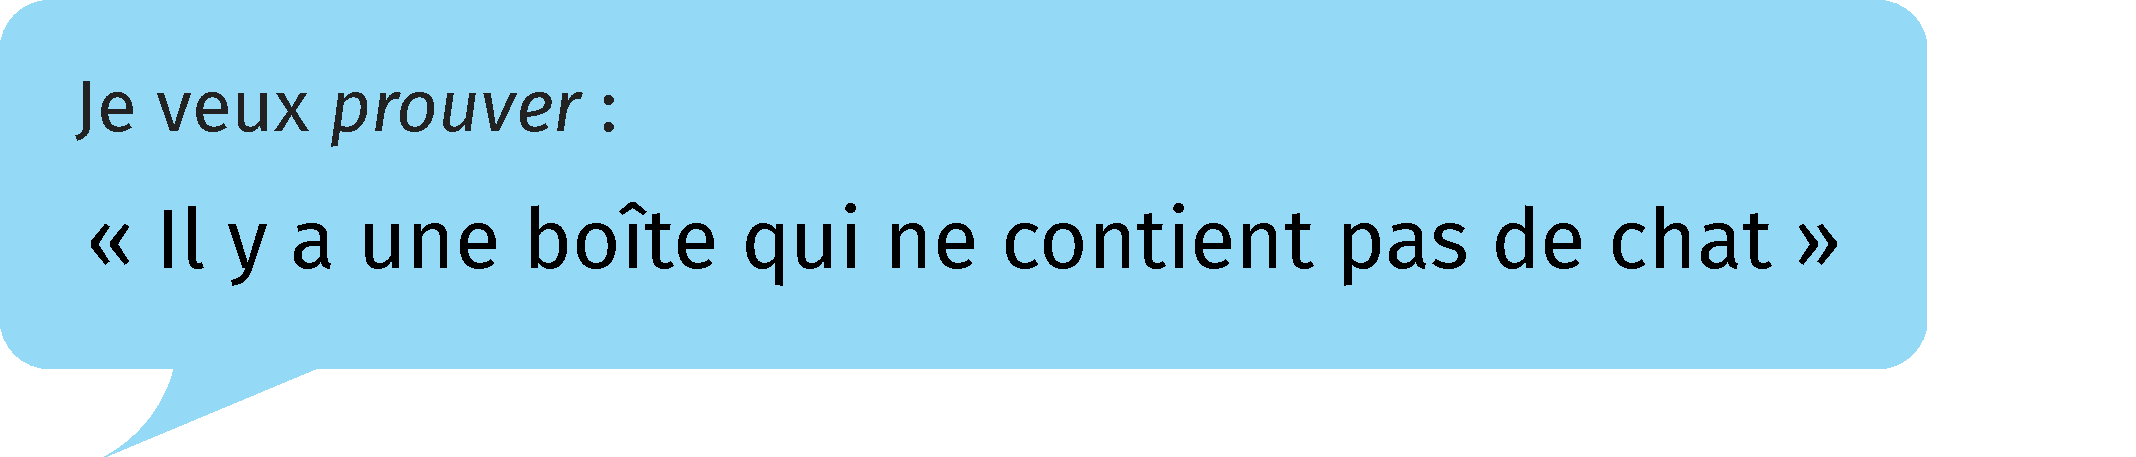
\includegraphics[width=0.8\textwidth]{conv-exists-fr.pdf}
  
\includegraphics[width=0.8\textwidth]{how-to-prove-fr.pdf}
\end{center}

La façon la plus simple de prouver que quelque chose existe est de fournir ce
que l'on appelle un \emph{témoin} d'existence. Ici, nous recherchons une boîte
qui ne contient pas de chat, il n'y a qu'une seule boîte sans chat, comme nous l'avons découvert lors de notre précédente épreuve, la troisième.

\begin{center}
  
\includegraphics[width=0.8\textwidth]{convo-take-third-fr.pdf}
  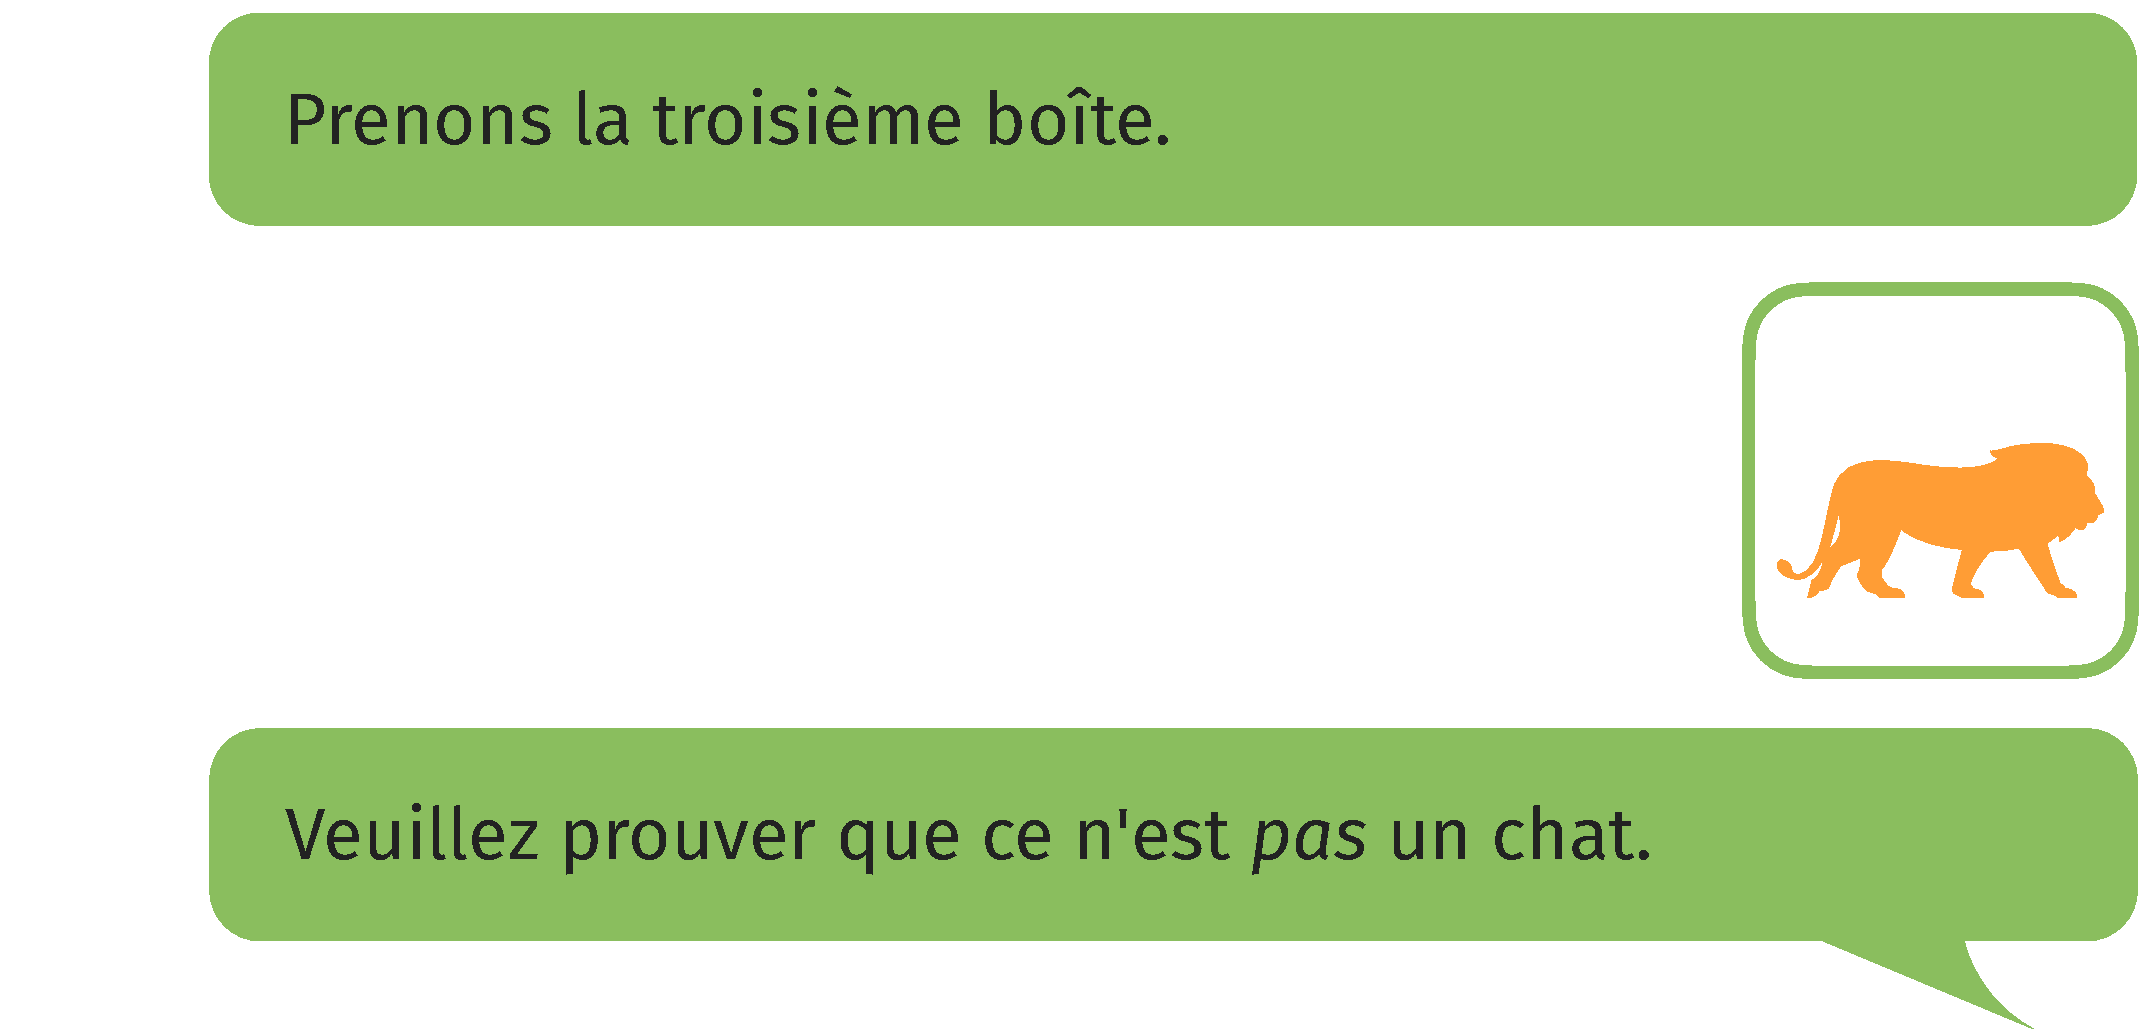
\includegraphics[width=0.8\textwidth]{convo-after-exists-fr.pdf}
  
\includegraphics[width=0.8\textwidth]{convo-trivial-fr.pdf}
  
\includegraphics[width=0.8\textwidth]{convo-indeed-fr.pdf}
  
\includegraphics[width=0.8\textwidth]{convo-proven-fr.pdf}
\end{center}

Un assistant de preuve nous aide donc à la fois à faire des preuves en
construisant des parties de la preuve lui-même et à vérifier qu'elles sont
correctes, par exemple en s'assurant qu'on n'a pas oublié un cas où nous avions
un lion plutôt qu'un chat.

Les assistants d'épreuve sont également intéressants et utiles pour d'autres
personnes que l'utilisateur qui fait la preuve. Disons que j'ai prouvé un
théorème compliqué en utilisant mon assistant de preuve préféré, les personnes
qui font confiance à mon assistant de preuve devront simplement lui demander
s'il est d'accord avec mon affirmation.
En fait, les assistants de preuve génèrent généralement ce que l'on appelle des
\emph{certificats} qui peuvent être vérifiés par d'autres sans avoir à
comprendre les détails de la preuve.

\begin{center}
  
\includegraphics[width=0.5\textwidth]{cerificate-fr.pdf}
\end{center}
\marginnote[-3cm]{
  L'image peut être trompeuse, je parle vraiment d'un objet concret que les gens
  peuvent analyser à l'aide de leur propre assistant de preuve pour vérifier
  qu'une preuve est bien valide.
}

Quand bien même, pourquoi devrions-nous faire confiance à l'assistant de
preuve ? Que pouvons-nous prouver exactement avec des assistant à la preuve ?
Et comment pouvons-nous les améliorer ?
Une partie de mon travail est centrée sur ces questions, et sur l'étude des
assistants de preuve basés sur ce que l'on appelle la théorie des types.

\section{Preuves, types et programmes}

Afin d'expliquer le titre ``Formalisation et méta-théorie de la théorie des
types'', j'ai besoin d'expliquer ce qu'est la \emph{théorie des types}.
Avant cela, je pense que je dois introduire la \emph{théorie de la preuve}
(\refch{proof-theory}) : l'étude des preuves elles-mêmes.
En effet, pour construire un assistant de preuve, il faut comprendre ce qu'est
une preuve, formellement, c'est-à-dire en termes très précis et non ambigus.

Il s'avère que certaines notions formelles de preuves ont des relations complexes avec la programmation comme nous le verrons dans le \refch{simple-types}.
L'idée est que les programmes peuvent être considérés comme des preuves et les
preuves comme des programmes.
Par exemple, la preuve qu'un proposition \(A\) implique la proposition \(B\)
est un programme qui prend une preuve de \(A\) en entrée et renvoie une preuve
de \(B\) en sortie.
Un tel programme est de type \(A \to B\). Les types sont un moyen de décrire les
données renvoyées par un programme. Les étudiants sont souvent amenés à écrire
la fameuse fonction de test d'une année bissextile qui, étant donnée une année
sous forme d'entier (décrit par le type \mintinline{ocaml}{int}), répond s'il
s'agit d'une année bissextile ou non. Cette information binaire --- oui ou non
--- est encodée dans ce que nous appelons des booléens
(\mintinline{ocaml}{bool}).
La correspondance de Curry-Howard indique que les programmes de type \(A\)
peuvent être considérés comme des preuves de la proposition \(A\) et vice-versa.

Danse le \refch{dependent-types}, je décris enfin ce que j'appelle la théorie
des types.
La théorie des types est un cadre qui tire parti de cette correspondance et est donc au cœur d'assistants de preuve bien connus tels que
\Coq~\sidecite[-1.3cm]{coq} et \Agda~\sidecite[-0.2cm]{norell2007towards}.
Je suis moi-même un utilisateur de \Coq et cette thèse est écrite en mettant
l'accent sur cet assistant de preuve et ses fondements.
Dans le \refch{usual-defs}, je décris les définitions habituelles qui
accompagnent la théorie des types.
J'explique comment nous pouvons raisonner dans un tel contexte avec plus que des
implications (\(\to\)).
\sidedeffr[-2.2cm]{Récurrence sur les entiers naturels}{%
  Si \(P(n)\) est une propriété sur l'entier naturel \(n\), et si
  \begin{enumerate}
    \item \(P(0)\);
    \item \(P(m)\) implique \(P(m+1)\) pour tout \(m\);
  \end{enumerate}
  alors on a \(P(n)\) pour tout \(n\).
}%
C'est là que j'introduis par exemple comment faire un récurrence sur des entier
naturels dans la théorie des types.

Le \refch{flavours} est dédié à différentes formulations et variantes de la
théorie des types. En effet, il n'y a pas qu'une seule théorie de ce genre.
Différentes théories de type ont des propriétés différentes, je répertorie les
plus importantes tout en disant quelle théorie possède quelle propriété dans un
tableau récapitulatif.

Le reste de la partie introductive se concentrera davantage sur la partie
``méta-théorie'' du titre. Alors que la théorie est l'endroit où l'on effectue now
preuves et où l'on écrit nos programmes, la méta-théorie est l'endroit où l'on raisonne sur la théorie elle-même !
Dans le \refch{models}, j'explique comment construire ce que l'on appelle des
modèles de théorie des types, qui consistent à interpréter la théorie et à lui
donner un sens --- ou une \emph{sémantique} --- à l'intérieur de la
méta-théorie. À la fin, je suggère comment la méta-théorie peut même être une
forme de théorie des types elle-même. La représentation de la théorie des types
en théorie des types est l'objet du \refch{formalisation} tandis que le
\refch{translations} se concentre sur la façon dont nous pouvons donner un sens à une théorie des types, en utilisant une autre théorie des types.

\section{Élimination de la \emph{reflection}}

Ensuite, nous avons la \arefpart{elim-reflection}.
Le titre peut fair peur, mais il tombe dans la catégorie ``que puis-je prouver
avec mon assistant de preuve ?'' Et ``comment puis-je améliorer les assistants
de preuve ?''

La théorie des types est à l'interface de la logique et de la programmation.
Traditionnellement, les langages de programmation sont conçus avec l'idée que,
à la fin, les programmes seront \emph{exécutés} ou \emph{évalués}. En d'autres
termes, les programmes \emph{calculent}.
Le calcul est également un élément important de la théorie des types. Le calcul
correspond à la simplification des preuves, mais surtout il incarne la notion de
\emph{constructivisme}. Supposons que, dans l'exemple précédent, vous prouvez
qu'il ``existe un chat avec un problème de gravité'', si vous exécutez cette
preuve, elle calculera et produira deux informations importantes: qui est le
chat fautif --- dans ce cas le noir dans la deuxième boîte --- et pourquoi il a
des problèmes de gravité (donnée comme une autre preuve qui correspondra à peu
près à montrer que le chat est à l'envers).

Le calcul est également utile lors de la réalisation de preuves.
Par exemple, \(2 + 2\) \emph{vaut} \(4\), donc pas besoin de transporter des
informations concernant la relation entre les deux. \(2 + 2\) s'évalue en \(4\),
donc deux ensembles de deux boîtes de chat correspond juste à un ensemble de
quatre boîtes de chat, et l'assistant de preuve le sait.

\marginnote[2cm]{
  Le calcul est \emph{dirigé}: \(2 + 2\) se simplifie, ou s'évalue, en
  \(4\), et pas l'inverse. \(2 + 2\) et \(3 + 1\) sont égaux parce que les deux
  s'évaluent en \(4\):
  \[
    2 + 2 \red 4 \redl 3 + 1
  \]
}
Il existe différents degrés de calcul qui peuvent être mis dans une théorie des
type, et on peut se demander quels impacts le calcul a sur la théorie.
Je présente un spectre de trois théories différentes. D'un côté, une théorie,
appelée théorie extentionnelle des types (ETT), qui est très libérale en ce qui
concerne le calcul en ce qu'elle identifie deux choses que si prouvées ou
supposées égales. Dans un tel contexte, le calcul n'est plus dirigé et nous
parlons simplement des choses comme étant \emph{égales}.
Ce principe, transformant une preuve en égalité, est appelé \emph{reflecion} de
l'égalité.
L'autre extrême est une théorie, appelée théorie faible des types (WTT), où nous
supprimons la notion même de calcul. Au milieu, nous avons la théorie
intentionnelle des types (ITT) qui a une notion de calcul ``usuelle'', définie
comme l'évaluation des fonctions. Cette dernière est à la base de \Coq et \Agda.

Ma contribution est une traduction de \acrshort{ETT} vers \acrshort{ITT} et
\acrshort{WTT}, montrant que le calcul n'est pas une propriété essentielle ---
bien que très pratique --- de la théorie des types du point de vue logique : en
effet, je montre que nous pouvons encore prouver les mêmes énoncés.
Cela signifie que nous pouvons raisonner sur la prouvabilité des énoncés dans
\acrshort{WTT}, qui est plus simple.
La traduction se fait dans la théorie des types elle-même --- dans ce cas \Coq
--- et fournit ainsi un programme transformant une preuve dans \acrshort{ETT} en
une preuve dans \acrshort{ITT} ou \acrshort{WTT} qui peut donc être utilisé
pour calculer de nouvelles preuves.

\section{Un vérificateur de typage pour \Coq, en \Coq}

Enfin, dans \arefpart {coq-in-coq}, je répondrai à la question ``Comment
peut-on augmenter la confiance dans un assistant de preuve ?'' En me concentrant
une fois de plus sur \Coq, je présente une vérification du noyau de \Coq, en
utilisant \Coq lui-même.

\Coq dispose d'un noyau, c'est-à-dire un programme assez petit qui vérifie que
les preuves sont bien correctes. La partie interactive de l'assistant de preuve,
ainsi que l'automatisation --- c'est-à-dire ce qui fait que l'assistant de
preuve trouve des preuves pour nous --- ne font pas partie du noyau et sont
plutôt construites au-dessus de lui.
Si vous voulez, la partie qui vérifie les certificats est distincte du reste et,
en tant que telle, est plus facile à étudier.

\begin{center}
  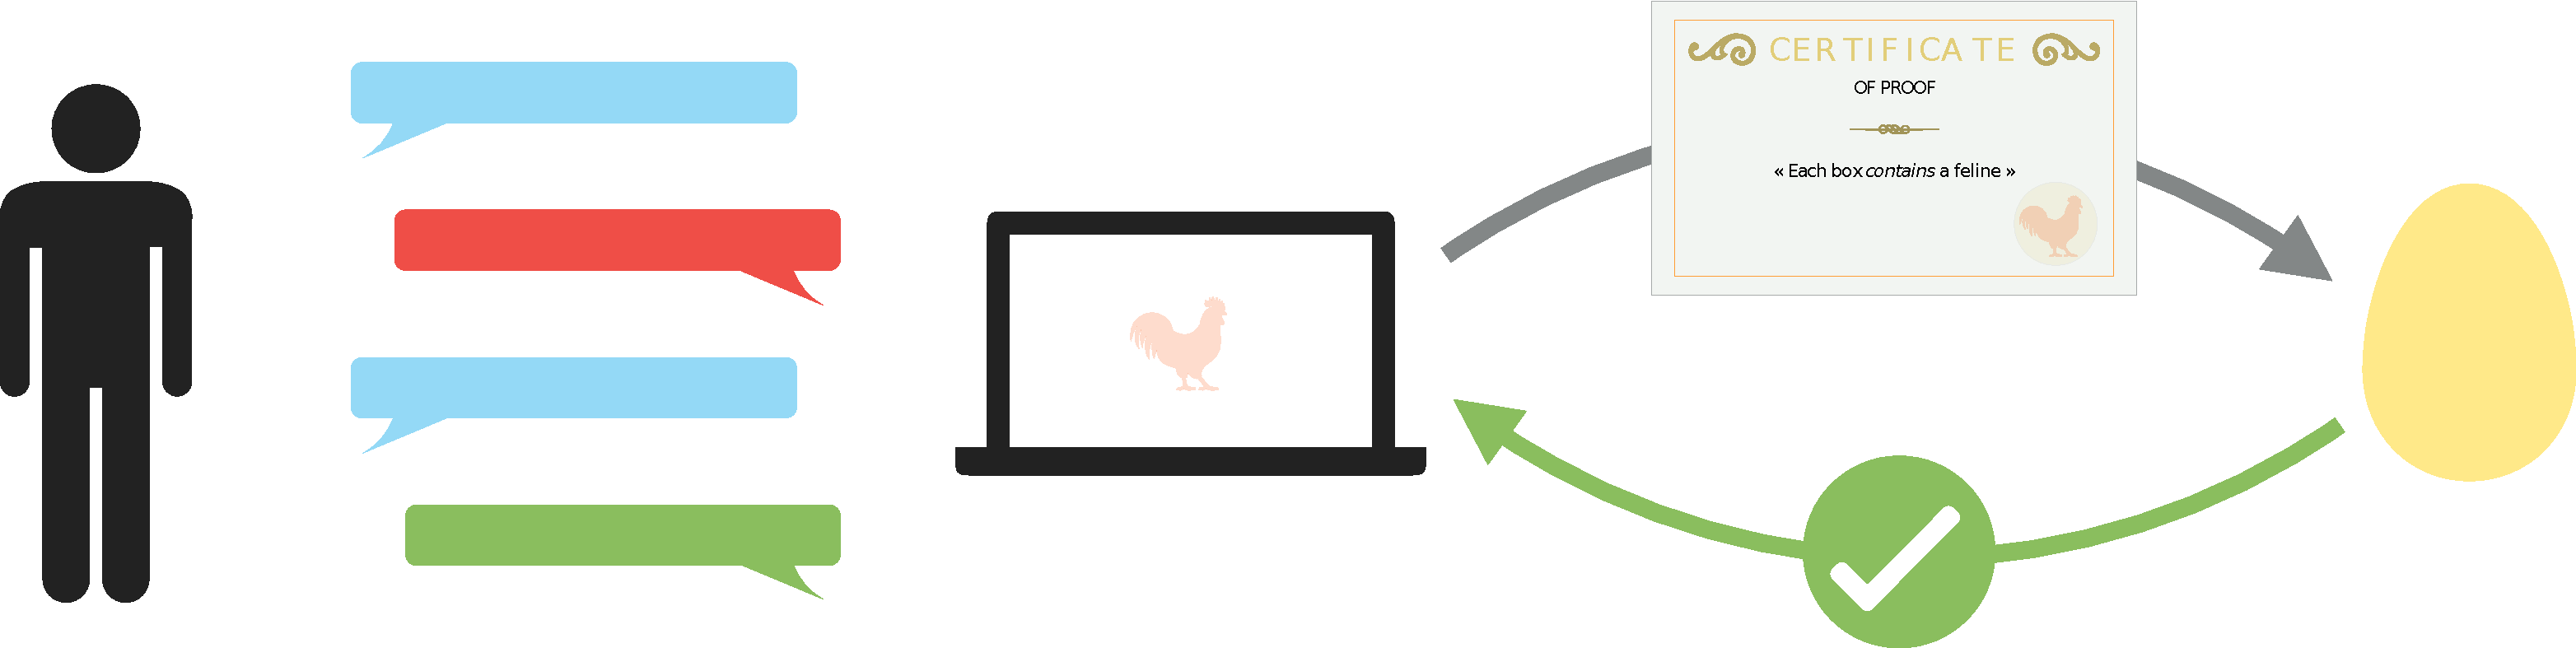
\includegraphics[width=0.9\textwidth]{chatbot-kernel.pdf}
\end{center}
\marginnote[-2.5cm]{
  L'œuf à droite représente le noyau. L'assistant de preuve lui envoie
  essentiellement le certificat qu'il a généré après discussion avec
  l'utilisateur et le noyau le valide (ou non).
}

Si l'assistant de preuve est défectueux, le certificat sera incorrect et rejeté
par le noyau. Tant que le noyau est correct, il n'est pas crucial que le reste
soit complètement correct. Certes, c'est plus agréable quand tout est correct,
mais seule l'exactitude du noyau est cruciale.
Comme je l'ai dit, des efforts sont faits pour garder le noyau aussi petit que
possible afin que des humains puissent l'inspecter et affirmer son exactitude.

Malheureusement, même un assistant de preuve aussi largement utilisé que \Coq
n'est pas exempt d'erreurs : un bogue critique a été trouvé à peu près chaque
année au cours des vingt dernières années. Ceux-ci sont généralement résolus
assez rapidement, mais leur simple existence est néanmoins gênante.
Une preuve incorrecte peut avoir des conséquences désastreuses. \Coq n'est pas
seulement utilisé pour prouver des théorèmes mathématiques, mais aussi pour
vérifier des programmes et s'assurer qu'ils ne planteront pas ou ne se
retrouveront pas dans des configurations indésirables. Ces programmes que nous
voulons vérifier sont souvent utilisés dans les parties critiques des logiciels,
par exemple dans les pilotes automatiques et les fusées, où la plus petite
erreur peut coûter des millions... et des vies.

Je fais partie d'un projet --- le projet \MetaCoq --- qui a pour but de
spécifier et vérifier le noyau de \Coq lui-même, dans \Coq. Cela signifie que
nous produisons un noyau séparé, entièrement écrit et vérifié dans \Coq qui peut
également vérifier les certificats indépendamment.

Lors de la vérification du noyau, nous devons nous fier aux propriétés
méta-théoriques de la théorie de \Coq. Malheureusement, toutes ne peuvent pas
être prouvés dans \Coq lui-même.
\marginnote[0.1cm]{
  Je parlerai des théorèmes d'incomplétude de Gödel dans le
  \nrefch{proof-theory}.
}%
Cela est dû aux théorèmes d'incomplétude de Gödel qui impliquent à peu près
qu'une théorie comme celle de \Coq ne peut pas prouver sa propre cohérence.
Ainsi, nous devons supposer certaines de ces propriétés méta-théoriques, en
particulier celles suffisamment fortes pour impliquer la cohérence de \Coq, donc
qui ne peuvent pas être prouvées.
Nous proposons donc un changement de paradigme : au lieu d'avoir un noyau
relativement petit auquel on fait confiance, nous nous appuyons sur une petite
base de propriétés supposées sur la théorie, théorie qui a été bien étudiée au
fil des années et qui ne souffre pas des bogues découverts dans l'implantation.
Il y a d'autres défis auxquels nous devons faire face, l'un d'entre eux est la
preuve que les définitions que nous fournissons pour construire le noyau sont
terminantes, cela a été beaucoup plus compliqué que prévu et cela nous a forcés
à rendre explicite plusieurs invariants qui sont implicites dans l'implantation
actuelle.

Dans l'ensemble, nous fournissons une spécification de \Coq, dans \Coq, avec
quelques propriétés sur la théorie que nous devons supposer. À partir de cela
nous vérifions la correction d'un noyau de \Coq alternatif.

\selectlanguage{english}